\section{Experiments}\label{sec:experiments}
For our experiments we plan and execute queries for three separate survey-based data sets.
We show that \ProjectName{} performs an order of magnitude better than traditional
base-table imputation and produces results of comparable quality, showing that our system is well suited for early dataset exploration.

\subsection{Data Sets}\label{subsec:datasets}
We collect three data sets for our experiments.
For all data sets, we selected a subset of the original attributes.
We also transform all data values to an integer representation by enumerating strings and transforming floating-point values into an appropriate range.

\subsubsection{CDC NHANES}
For our first set of experiments, we use survey data collected by the 
U.S. Centers for Disease Control and Prevention (CDC). We
experiment on a set of tables collected as part of the 2013--2014 National
Health and Nutrition Examination Survey (NHANES), a series of studies
conducted by the CDC on a national sample of several thousand individuals~\cite{cdc-data}.
The data consists of survey responses, physical examinations, and laboratory
results, among others.

There are 6 tables in the NHANES data set. We use three tables for our experiments: demographic information of subjects (\texttt{demo}), physical exam results (\texttt{exams}), and laboratory exam results (\texttt{labs}).

The original tables have a large number of attributes, in some cases providing more granular test results or alternative metrics.
We focus on a subset of the attributes for each table to simplify the presentation and exploration of queries.
\Cref{table:nhanes-description} shows the attributes selected, along with the percentage of \nullv{} values for each attribute.
For readability, we have replaced the NHANES attribute names with self-explanatory attribute names.

\begin{table*}
  \centering
  \begin{subtable}{0.3\textwidth}
    \centering
    \begin{tabular}{llr}
\toprule
\textbf{Attribute} &  \textbf{\% Missing} \\
\midrule
age\_months &      93.39 \\
age\_yrs &       0.00 \\
gender &       0.00 \\
id &       0.00 \\
income &       1.31 \\
is\_citizen &       0.04 \\
marital\_status &      43.30 \\
num\_people\_household &       0.00 \\
time\_in\_us &      81.25 \\
years\_edu\_children &      72.45 \\
\bottomrule
\end{tabular}

    \caption{Demographics (\texttt{demo}). \demorows{} rows.}
  \end{subtable}\quad\begin{subtable}{0.3\textwidth}
    \centering
    \begin{tabular}{lS[table-format=2.2]}
\toprule
\textbf{Attribute} &  \textbf{Missing} \\
\midrule
albumin &      17.95\ \% \\
blood\_lead &      46.86\ \% \\
blood\_selenium &      46.86\ \% \\
cholesterol &      22.31\ \% \\
creatine &      72.59\ \% \\
hematocrit &      12.93\ \% \\
id &       0.00\ \% \\
triglyceride &      67.94\ \% \\
vitamin\_b12 &      45.83\ \% \\
white\_blood\_cell\_ct &      12.93\ \% \\
\bottomrule
\end{tabular}

%%% Local Variables:
%%% mode: latex
%%% TeX-master: "../main"
%%% End:

    \caption{Laboratory Results (\texttt{labs}). \labexrows{} rows.}
  \end{subtable}\quad\begin{subtable}{0.3\textwidth}
    \centering
    \begin{tabular}{llr}
\toprule
 Table &                Attribute &  \% Missing \\
\midrule
 exams &        arm\_circumference &       5.22 \\
 exams &      blood\_pressure\_secs &       3.11 \\
 exams &  blood\_pressure\_systolic &      26.91 \\
 exams &          body\_mass\_index &       7.72 \\
 exams &                cuff\_size &      23.14 \\
 exams &       head\_circumference &      97.67 \\
 exams &                   height &       7.60 \\
 exams &                       id &       0.00 \\
 exams &      waist\_circumference &      11.74 \\
 exams &                   weight &       0.92 \\
\bottomrule
\end{tabular}

    \caption{Physical Results (\texttt{exams}). \labexrows{} rows.}
  \end{subtable}
  \caption{Percentage of values missing in the CDC NHANES 2013--2014 data.}\label{table:nhanes-description} 
\end{table*}

\subsubsection{freeCodeCamp 2016 New Coder Survey}
For our second set of experiments, we use data collected by freeCodeCamp, an open-source
community for learning to code, as part of a survey of new software
developers~\cite{fcc-data}.  The \textit{2016 New Coder Survey} consists of responses by
over 15,000 people to 48 different demographic and programming-related questions.  The
survey targeted users who were related to coding organizations.

We use a version of the data that has been pre-processed, but where missing values remain.
For example, 46.6\% of \textit{commutetime} responses are missing. However, it is worth
noting that some of the missing values are also expected, given the way the data has been
de-normalized. For example, \textit{bootcamploanyesno}, a binary attribute encoding whether
a respondent had a loan for a bootcamp, is expected to be \nullv{} for participants who did not
attend a bootcamp.

We choose a subset of 17 attributes, which are shown in~\Cref{table:fcc-description} along
with the percentage of missing values.

\begin{table}
  \centering
  \begin{tabular}{lr}
\toprule
            \textbf{Attribute} &  \textbf{\% Missing} \\
\midrule
age &      12.85 \\
attendedbootcamp &       1.54 \\
 bootcampfinish &      94.03 \\
 bootcampfulljobafter &      95.93 \\
 bootcamploanyesno &      94.02 \\
 bootcamppostsalary &      97.89 \\
childrennumber &      83.65 \\
citypopulation &      12.74 \\
commutetime &      46.61 \\
countrycitizen &      12.59 \\
gender &      12.00 \\
hourslearning &       4.34 \\
income &      53.08 \\
moneyforlearning &       6.02 \\
monthsprogramming &       3.88 \\
schooldegree &      12.43 \\
studentdebtowe &      77.50 \\
\bottomrule
\end{tabular}

  \caption{Percentage of values missing in the freeCodeCamp Survey data (\texttt{fcc}).}\label{table:fcc-description} 
\end{table}

\subsubsection{American Community Survey}
For our final experiment, we run a simple aggregate query over data from the American
Community Survey (ACS), a comprehensive survey conducted by the U.S.
Census Bureau. We use a cleaned version of the 2012 Public Use Microdata Sample (PUMS) data,
which we then artificially dirty by replacing 40\% of the values uniformly at random with
\nullv{} values.
The final dataset consists of 671,153 rows and 37 integer columns.

\subsection{Queries}
We collect a set of queries (\Cref{tbl:queries}) that we think are interesting to plan.
We believe that they could reasonably be written by a user in the course of data analysis.

The queries consist not only of projections and selections, but also
interesting joins and aggregates. Our aim was to craft meaningful queries that would
provide performance figures relevant to practitioners using similar datasets.
\review{
Our benchmark queries performed well for both cases of \texttt{AVG} and \texttt{COUNT} aggregates, 
so we expect \ProjectName{} to perform similarly for \texttt{SUM}, with 
errors proportional to the fraction of relevant tuples retrieved and the \texttt{AVG} value estimated.}

%Our first set of queries is on the CDC data (\Cref{fig:queries-cdc}).
%\Cref{q1} calculates the average cuff size for individuals based on their income data, with a constraint on height.
%\Cref{q2} compares creatine levels for individuals with low, medium, and high incomes and above a certain weight.
%\Cref{q3} extracts the average blood lead levels for children under 6 years of age.
%\Cref{q4} calculates the average systolic blood pressure, by gender, for subjects with a body mass index indicating obesity. 
%\Cref{q5} calculates the average waist circumference for subjects above a certain height and weight.
%
%Our second set of queries is on the freeCodeCamp data (\Cref{fig:queries-fcc}).
%\Cref{q6} calculates the average income for higher-income survey participants, grouped by their bootcamp attendance.
%\Cref{q7} estimates the average commute time of women from the United States who participated.
%\Cref{q8} calculates the average amount of student debt based on school degree for survey participants who have student debt.
%\Cref{q9} joins the freeCodeCamp data with a table provided by the World Bank which summarizes GDP per-capita across various countries~\cite{worldbank-data}.
%The query calculates the average GDP per-capita by grouping 18+ year old participants who attended bootcamp versus those who did not.

\begin{table*}
  \centering
  \newcounter{queryno}
\begin{tabular}{cl}
\toprule
\# & \multicolumn{1}{c}{Queries on CDC data} \\
\midrule
1 & 
\begin{minipage}{6in}
\begin{lstlisting}[breaklines]
SELECT income, AVG(cuff_size) FROM demo, exams 
WHERE demo.id = exams.id AND height >= 150 GROUP BY income;
\end{lstlisting}
\end{minipage}\refstepcounter{queryno}\label[query]{q1} \\
2 & 
\begin{minipage}{6in}
\begin{lstlisting}[breaklines]
SELECT income, AVG(creatine) FROM demo, exams, labs 
WHERE demo.id = exams.id AND exams.id = labs.id AND income >= 13 AND income <= 15 AND weight >= 63 GROUP BY income;
\end{lstlisting}
\end{minipage}
\refstepcounter{queryno}\label[query]{q2} \\
3 & 
\begin{minipage}{6in}
\begin{lstlisting}[breaklines]
SELECT AVG(blood_lead) FROM demo, exams, labs 
WHERE demo.id = labs.id AND labs.id = exams.id AND age_yrs <= 6;
\end{lstlisting}
\end{minipage}\refstepcounter{queryno}\label[query]{q3}\\
4 & 
\begin{minipage}{6in}
\begin{lstlisting}[breaklines]
SELECT gender, AVG(blood_pressure_systolic) FROM demo, labs, exams 
WHERE demo.id = labs.id AND labs.id = exams.id AND body_mass_index >= 30 GROUP BY gender;
\end{lstlisting}
\end{minipage}\refstepcounter{queryno}\label[query]{q4}\\
5 & 
\begin{minipage}{6in}
\begin{lstlisting}[breaklines]
SELECT AVG(waist_circumference) FROM demo, exams 
WHERE demo.id = exams.id AND height >= 150 AND weight >= 100;
\end{lstlisting}
\end{minipage}\refstepcounter{queryno}\label[query]{q5}\\
  \midrule
\# & \multicolumn{1}{c}{Queries on freeCodeCamp data} \\
\midrule
6 & 
\begin{minipage}{6in}
\begin{lstlisting}[breaklines]
SELECT attendedbootcamp, AVG(income) FROM fcc
WHERE income >= 50000 GROUP BY attendedbootcamp;
\end{lstlisting}
\end{minipage}\refstepcounter{queryno} \label[query]{q6} \\
7 & 
\begin{minipage}{6in}
\begin{lstlisting}[breaklines]
SELECT AVG(commutetime) FROM fcc
WHERE gender = "female" AND countrycitizen = "United States";
\end{lstlisting}
\end{minipage}\refstepcounter{queryno} \label[query]{q7} \\
8 & 
\begin{minipage}{6in}
\begin{lstlisting}[breaklines]
SELECT schooldegree, AVG(studentdebtowe) FROM fcc
WHERE studentdebtowe > 0 GROUP BY schooldegree;
\end{lstlisting}
\end{minipage}\refstepcounter{queryno} \label[query]{q8}\\
9 & 
\begin{minipage}{6in}
\begin{lstlisting}[breaklines]
SELECT attendedbootcamp, AVG(gdp_per_capita) FROM fcc, gdp
WHERE fcc.countrycitizen = gdp.country AND age >= 18
GROUP BY attendedbootcamp;
\end{lstlisting}
\end{minipage}\refstepcounter{queryno} \label[query]{q9}\\
\bottomrule
\end{tabular}

%%% Local Variables:
%%% mode: latex
%%% TeX-master: "main"
%%% End:

  \vspace{1ex}
  \caption{Queries used in our experiments.}\label{tbl:queries}
\end{table*}

%\begin{table*}
%  \centerfloat
%  \begin{tabular}{cSSSSSSS}
\toprule
\multicolumn{2}{c}{} & \multicolumn{2}{c}{Imputed ($\alpha=0.0$)} & \multicolumn{2}{c}{Imputed ($\alpha=1.0$)} \\
\cmidrule(r){3-4}
\cmidrule(l){5-6}
\# & \multicolumn{1}{c}{Base error} & \multicolumn{1}{c}{Error} & \multicolumn{1}{c}{Time (s)} & \multicolumn{1}{c}{Error} & \multicolumn{1}{c}{Time (s)} \\
\midrule
\ref{q1} & 5.25e+03 & 0.00e+00 & 1.723 & -3.60e+03 & 11.008 \\
\ref{q2} & 3.38e+04 & 0.00e+00 & 1.748 & -3.37e+04 & 10.144 \\
\ref{q3} & 9.32e-04 & 0.00e+00 & 1.732 & 2.54e-02 & 33.04 \\
\ref{q4} & 1.78e+05 & 0.00e+00 & 1.778 & -1.55e+05 & 21.013 \\
\ref{q5} & 9.89e-04 & 0.00e+00 & 1.712 & 9.89e-02 & 7.981 \\
\ref{q6} & 1.01e-02 & 0.00e+00 & 1.982 & 1.13e-02 & 52.309 \\
\ref{q7} & 0.00e+00 & 0.00e+00 & 43M49.786 & 0.00e+00 & 5.946 \\
\ref{q8} & 0.00e+00 & 0.00e+00 & 1.776 & 0.00e+00 & 3.172 \\
\ref{q9} & \multicolumn{1}{c}{--} & \multicolumn{1}{c}{--} & 1.919 & \multicolumn{1}{c}{--} & 2M40.384 \\
\ref{q10} & \multicolumn{1}{c}{--} & \multicolumn{1}{c}{--} & 0.01 & \multicolumn{1}{c}{--} & 7.786 \\
\ref{q11} & \multicolumn{1}{c}{--} & \multicolumn{1}{c}{--} & 0.007 & \multicolumn{1}{c}{--} & 0.103 \\
\ref{q12} & 0.00e+00 & 0.00e+00 & 0.008 & 1.00e-02 & 0.175 \\
\ref{q13} & \multicolumn{1}{c}{--} & \multicolumn{1}{c}{--} & 0.407 & \multicolumn{1}{c}{--} & 0.4 \\
\ref{q14} & 0.00e+00 & 0.00e+00 & 0.752 & 4.37e-01 & 1M14.221 \\
\bottomrule
\end{tabular}

%    \caption{Base error, percent change in error and and running time for queries
%    with different imputation levels. Base error is the root-mean-square error (RMSE) between the query on clean
%    data and the query run on dirty data without imputation. Change in error is relative to the base error.}
%  \label{fig:experiments}
%\end{table*}

\review{
\subsection{Results}\label{sec:results}

We evaluate \ProjectName{} optimizing for quality ($\alpha=0$), optimizing for performance
($\alpha=1$), and targeting a balance of each ($\alpha = 0.5$). As a baseline, we fully impute the tables
used by each query and then run the query on the imputed tables, simulating the process that
an analyst would follow to apply existing imputation techniques.

\textbf{Runtime vs. Base-table Imputation}\quad \Cref{fig:runtimes} summarizes the performance results. The quality-optimized
queries, with runtimes ranging from \runtimetreelowzero{} to \runtimetreehighzero{}, are an
order-of-magnitude faster than the baseline, with runtimes ranging from
\runtimetreelowbase{} to \runtimetreehighbase{}. We get another order-of-magnitude speedup when
optimizing for performance, achieving runtimes as low as \runtimetreelowone{} to
\runtimetreehighone{}. These speedups, ranging widely from \lowxalphazero{}x to 
\highxalphaone{}x, depending on $\alpha$ and query, constitute significant workflow improvements
for the analyst.

\begin{figure}
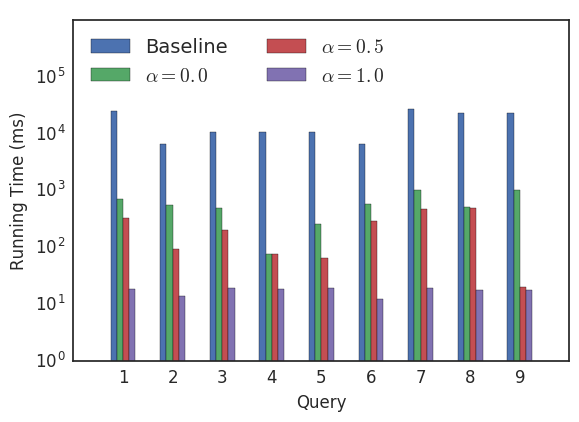
\includegraphics[width=\columnwidth]{figures/running_times_combined_bar.png}
\caption{Runtimes for the queries in~\Cref{tbl:queries} using reference
    chained-equation decision trees algorithm. Using $\alpha=0$, \ProjectName{}
    is run at the highest quality setting, while with $\alpha=1$, performance
    is prioritized. Each query and each value of $\alpha$ was run 200 times.}
\label{fig:runtimes}
\end{figure}

%\Cref{fig:plantimes} provides a summary of the planning times for each of the queries.
%We exclude the planning time for queries that impute at base table, as that requires no
%planning. 

% The one-standard-deviation
%intervals around the mean planning time often overlap, suggesting the planning component is
%constant in $\alpha$.

%\begin{figure}
%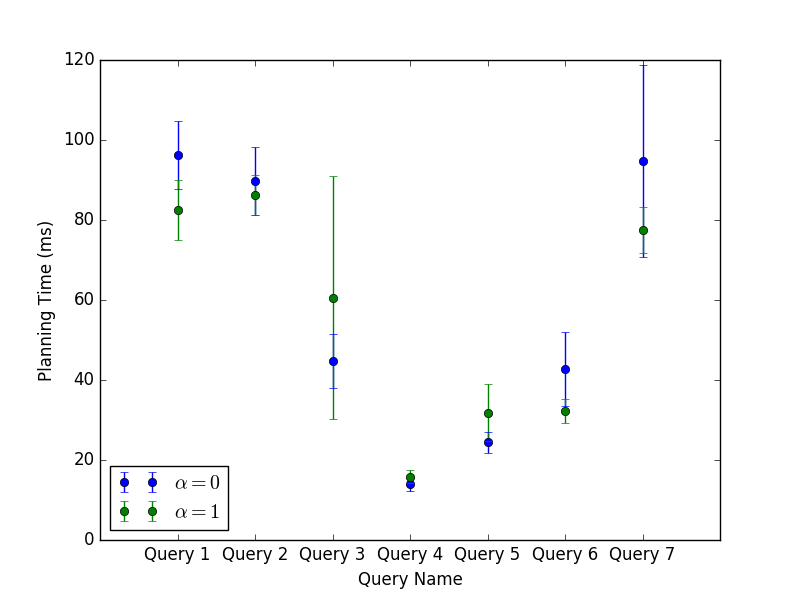
\includegraphics[width=\columnwidth]{figures/planning_times_imputedb.png}
%\caption{Planning times for each query}
%\label{fig:plantimes}
%\end{figure}

\textbf{Accuracy vs. Base-table Imputation (AVG)}\quad \Cref{table:smape} shows the Symmetric-Mean-Absolute-Percentage-Error (SMAPE)~\cite{Makridakis2000451} for \ProjectName{}'s query results compared to the baseline, using the reference chained-equation decision trees model.
This measures the error introduced by on-the-fly imputation as compared to full imputation on the base tables.
This comparison is the relevant one in practice --- an analyst would only be considering the trade-offs in imputation quality and time in the first place for dirty input data, for which ground truth is unavailable.

To calculate SMAPE for each $\alpha$,
we compute tuple-wise absolute percentage deviations within each iteration of each query, and
average this value over all iterations.
Relative errors of query results, when optimizing for quality
($\alpha=0$), are low --- between \lowsmapealphazero{} and
\highsmapealphazero{}\% --- indicating that on-the-fly imputation produces
results similar to the baseline. When optimizing for performance ($\alpha=1$),
relative errors can be modestly higher --- up to \highsmapealphaone{}\% in the
worst case, as this approach most closely corresponds to dropping all
\nullv{}s. Thus, it is important to recognize the trade-offs between quality and
performance for a specific use case.

\textbf{Accuracy vs. Base-table Imputation (COUNT)}\quad
We also calculate the number of tuples used to produce each aggregate output.
The count fraction columns in \Cref{table:smape} show the number of tuples in the aggregate for $\alpha = 0$ and $\alpha = 1$ as a fraction of the number of tuples used when running the query on the imputed base table.
This shows that when optimizing for performance, not quality, many tuples are dropped due to
insertion of $\delta$ operators.
Even in cases where the SMAPE reduction from $\alpha = 1$ and $\alpha = 0$ is small
(\Cref{q2} and \Cref{q6}) the tuple count is significantly different.
In these cases, the aggregate value is not significantly impacted by the missing data. In
particular, if values are missing completely at random,
the aggregate should not be affected.
However, if the missing data is biased then the aggregate will have a significant error.
This highlights a challenge for a user handling data imputation traditionally: it is unclear if the missing data will have a large or small negative impact on their analysis until they have paid the cost of running it.

By using \ProjectName{} this cost can be lowered significantly. We can also trivially extend \ProjectName{} to warn users when the query chosen for execution has a high
$\textsc{Penalty}$ estimate, along with the number of tuples that have been dropped (after execution), so that situations with high potential for skewed results can be identified by the user.

\textbf{Alternate Imputation Methods}\quad
We also experiment with mean-value imputation and hot deck imputation
(\Cref{sec:imputation}). In our implementation of mean-value imputation, to facilitate
non-blocking operation within the iterator model, we estimate the column mean from base
table histograms. Therefore, imputed values are identical no matter where the operator is
placed in the query plan (relative errors are $0$). Runtimes are in the range of
\runtimemeanlow{} to \runtimemeanhigh{} for queries using \ProjectName{}, as compared to
\runtimemeanlowbase{} to \runtimemeanhighbase{} when imputing on the base table.  Here, the
time cost of the imputation is low no matter how many tuples need to be imputed.  

In hot deck imputation, runtimes are also similar across $\alpha$, ranging from
\runtimehotdecklow{} to \runtimehotdeckhigh{} using dynamic imputation, as compared to
\runtimehotdecklowbase{} to \runtimehotdeckhighbase{} when imputing on the base table. In
this case, the cost of buffering tuples and sampling at random is negligible compared to the
rest of query execution. Relative errors using hot deck are close to zero, ranging from
\smapehotdecklow{}--\smapehotdeckhigh{}\%. (The exception is \Cref{q8} with $\alpha=1$, which has error
of \smapehotdeckhighoutlier{}\% and exhibits significant skew.) Since the baseline, in these
cases, is hot deck imputation on the base table, it is skew in the distributions arising from
filters and joins that often leads to larger errors. Indeed, \ProjectName{} yields
larger benefit when using relatively sophisticated, higher quality imputation algorithms as
opposed to simpler strategies that would even be quick to implement on the base table.

\textbf{Pareto Frontiers}\quad
\Cref{fig:pareto-frontiers} shows the final Pareto frontiers produced by the planner for \Cref{q1} and \Cref{q6}. These are the resulting set of plans after pruning dominated plans throughout our algorithm
and encapsulate the possible trade-offs that the user can make in choosing a final plan for execution. The frontier is available at the end of the planning stage and
can be exposed to the user to guide their workflow.

\begin{table}
\centering
\begin{tabular}{rrr}
\toprule
 Query &  \textbackslashalpha &  SMAPE \\
\midrule
     0 &     0.0 &   0.47 \\
     0 &     1.0 &   0.15 \\
     1 &     0.0 &   0.28 \\
     1 &     1.0 &   0.40 \\
     2 &     0.0 &   0.00 \\
     2 &     1.0 &   0.00 \\
     3 &     0.0 &   0.03 \\
     3 &     1.0 &   0.22 \\
     4 &     0.0 &  11.18 \\
     4 &     1.0 &    NaN \\
     5 &     0.0 &   0.79 \\
     5 &     1.0 &   1.93 \\
     6 &     0.0 &   0.00 \\
     6 &     1.0 &   0.03 \\
     7 &     0.0 &   0.82 \\
     7 &     1.0 &  35.44 \\
     8 &     0.0 &   0.23 \\
     8 &     1.0 &   0.31 \\
     9 &     0.0 & 100.00 \\
     9 &     1.0 & 100.00 \\
\bottomrule
\end{tabular}

\caption{Symmetric-Mean-Absolute-Percentage-Error for queries run under different $\alpha$ parameterizations, as compared to the baseline.
Queries optimized
    for quality ($\alpha=0$) generally achieve lower error than queries optimized for
    efficiency ($\alpha=1$). With ($\alpha=0.5$), an intermediate plan may be chosen if
    available.
    The count fraction column shows the number of tuples used in calculating each aggregate
     as a fraction of the number of tuples used when running the same query after imputing on the base table.
    A lower count share reflects more potential for errors.}
\label{table:smape}
\end{table}

\begin{figure}
\centering
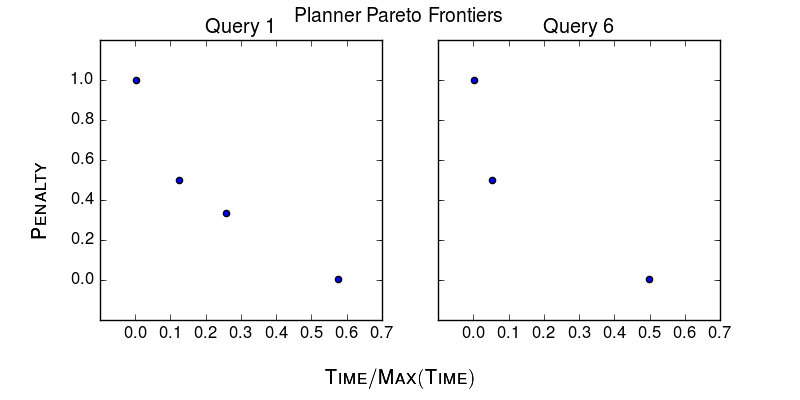
\includegraphics[scale=0.4]{figures/pareto_frontiers_plot.png}
\caption{\review{
    \ProjectName{}'s final planner Pareto frontier for \Cref{q1} and \Cref{q6}. 
    For clarity, we have removed from the plot plans that provide nearly indistinguishable trade-offs in either dimension.
}
\label{fig:pareto-frontiers}
}
\end{figure}

\textbf{Planning Times}\quad
Planning times for our benchmark queries are reasonable, with mean planning times across the
benchmark queries ranging from \planningtimelow{} to \planningtimehigh{}, and ranging from
\planningtimelowpct{} to \planningtimehighpct{}\% of total runtime. In 99\% of individual
cases, the optimizer returned a query plan within \planningtimepninetynine{}. The choice of
$\alpha$ has no impact on planning times, because query selection is done after collecting
the Pareto frontier.

\textbf{Approximate Pareto Sets}\quad
However, \ProjectName{}'s planning algorithm is still exponential in the number of joins in the plan, and the use of Pareto sets exacerbates this exponential growth.
We explored the limits of our planning algorithm by constructing a series of queries with increasing number of joins over the CDC tables.
Planning times for queries involving 1--5 joins---a practical value for  real world exploratory queries---are less than 1 second.
We extended \ProjectName{} to support an approximation of Pareto sets to improve planning times for queries with 6 or more joins. Approximate Pareto sets
displayed a reduction in planning time linear with respect to the reduction in size of the final frontier. For queries with 6--8 joins, approximate sets achieved a reduction
in planning time between 14\% and 23\%, on average. Users can increase the level of approximation to reduce planning times further.

\textbf{Imputation on Large Data}\quad
In many real-world cases, applying imputation to an entire dataset is prohibitively expensive.
For example, if we run chained-equation decision trees imputation on the full ACS dataset, it completes in \acsbaseresultminutes{}.

In contrast, \ProjectName{} executes the query \lstinline{SELECT AVG(c0) FROM acs} over the ACS dataset (also using chained-equation decision trees imputation) in \acsimputedbzeroresult{} when optimizing for quality and \acsimputedboneresult{} when optimizing for runtime. 
Given the runtime difference, we can run approximately 5,000 queries before taking more time than full imputation.
The performance difference comes from the fact that \ProjectName{} only needs to perform imputation on the single column required by the query.
Adding selection predicates would further reduce the query runtime by reducing the amount of required imputation.
An analyst could do the same, but tracking the required imputations would get increasingly complicated as the queries became more complex.
This highlights the benefit of using our system for early data exploration.
}


%\subsubsection{Planning Times}
%\begin{figure}
%\centering
%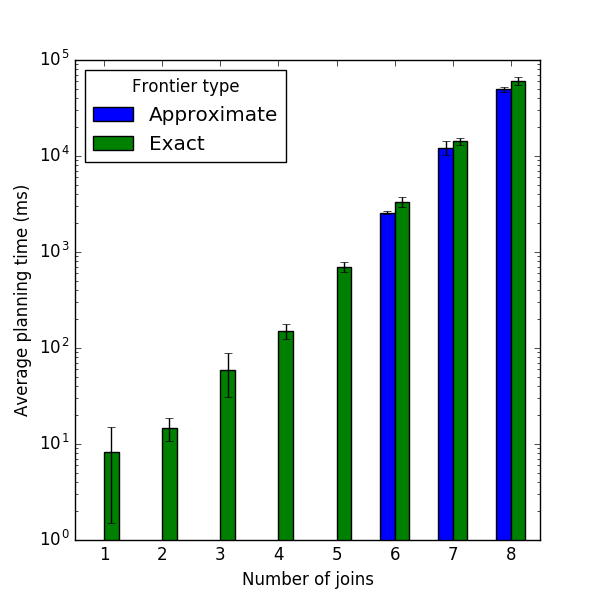
\includegraphics[scale=0.4]{figures/planning_times_plot.png}
%\caption{Planning times are sub-second for up to 5 joins. For more joins, we implement an approximation to Pareto sets. Users can increase the level of
%approximation for more aggressive planning reductions.
%}
%\label{fig:planning-times}
%\end{figure}
%\todobox{Jose: I'm not a fan of this line, I would remove}{Furthermore, at that point, it may make more sense to specify a coherent model over the entire base table instead.}

%%% Local Variables:
%%% mode: latex
%%% TeX-master: "main"
%%% End:
